\section*{Задание 1. Свободное движение}

Рассмотрим систему 2-го порядка, заданную дифференциальным уравнением
\begin{equation}
    \ddot y +a_1\dot y+a_0=u.
\end{equation}
Сделаем некоторые преобразования для структурной схемы, которую можно
увидеть в рисунке \ref{fig:task_1_slx} (начальные условия задаются в двух
последних интеграторах):
\begin{equation*}
    \begin{array}{c}
        p^2[y]+p[a_1y]+a_0=u,\\[2mm]
        y=\frac{1}{p^2}[u-a_0-a_1\dot y].
    \end{array}
\end{equation*}
Для каждого из вариантов задано по шесть наборов значений корней 
характеристического уравнения $\lambda_1$ , $\lambda_2$ и начальных условия 
$y(0), \dot y(0)$. Чтобы вычислить коэффициенты $a_1$ и $a_0$, 
воспользуемся формулами $a_1=-\lambda_1-\lambda_2$, $a_0=\lambda_1\lambda_2$.
Это все, а так же аналитические решения свободного движения можно увидеть 
в таблице \ref{tab:values}.

\begin{table}[h!]
    \centering
    \begin{tabular}{|c|c|c|c|c|c|c|c|}
    \hline
    \text{№} & $\lambda_1$ & $\lambda_2$ & $y(0)$ & $\dot{y}(0)$ & $a_0$ & $a_1$ & $y_\text{СВ}(t)$\\
    \hline
    1 & $-3$ & $-1.5$ & $1$ & $0$ & $4.5$ & $4.5$ & $2/9e^{-4.5t}+t-11/9$ \\
    \hline
    2 & $-1.2 + j10$ & $-1.2 - j10$ & $1$ & $0$ & $101.44$ & $2.4$ & \\
    \hline
    3 & $j10$ & $-j10$ & $1$ & $0$ & $100$ & $0$ & \\
    \hline
    4 & $1.2 + j10$ & $1.2 - j10$ & $0.05$ & $0$ & $101.44$ & $-2.4$ & \\
    \hline
    5 & $3$ & $1.5$ & $0.05$ & $0$ & $4.5$ & $-4.5$ & \\
    \hline
    6 & $-0.8$ & $0.8$ & $0$ & $0.1$ & $-0.64$ & $0$ & \\
    \hline
    \end{tabular}
    \caption{\label{tab:values}Таблица корнями характеристического уравнения, начальными условиями и коэффициентами.}
\end{table}

\begin{figure}
    \centering
    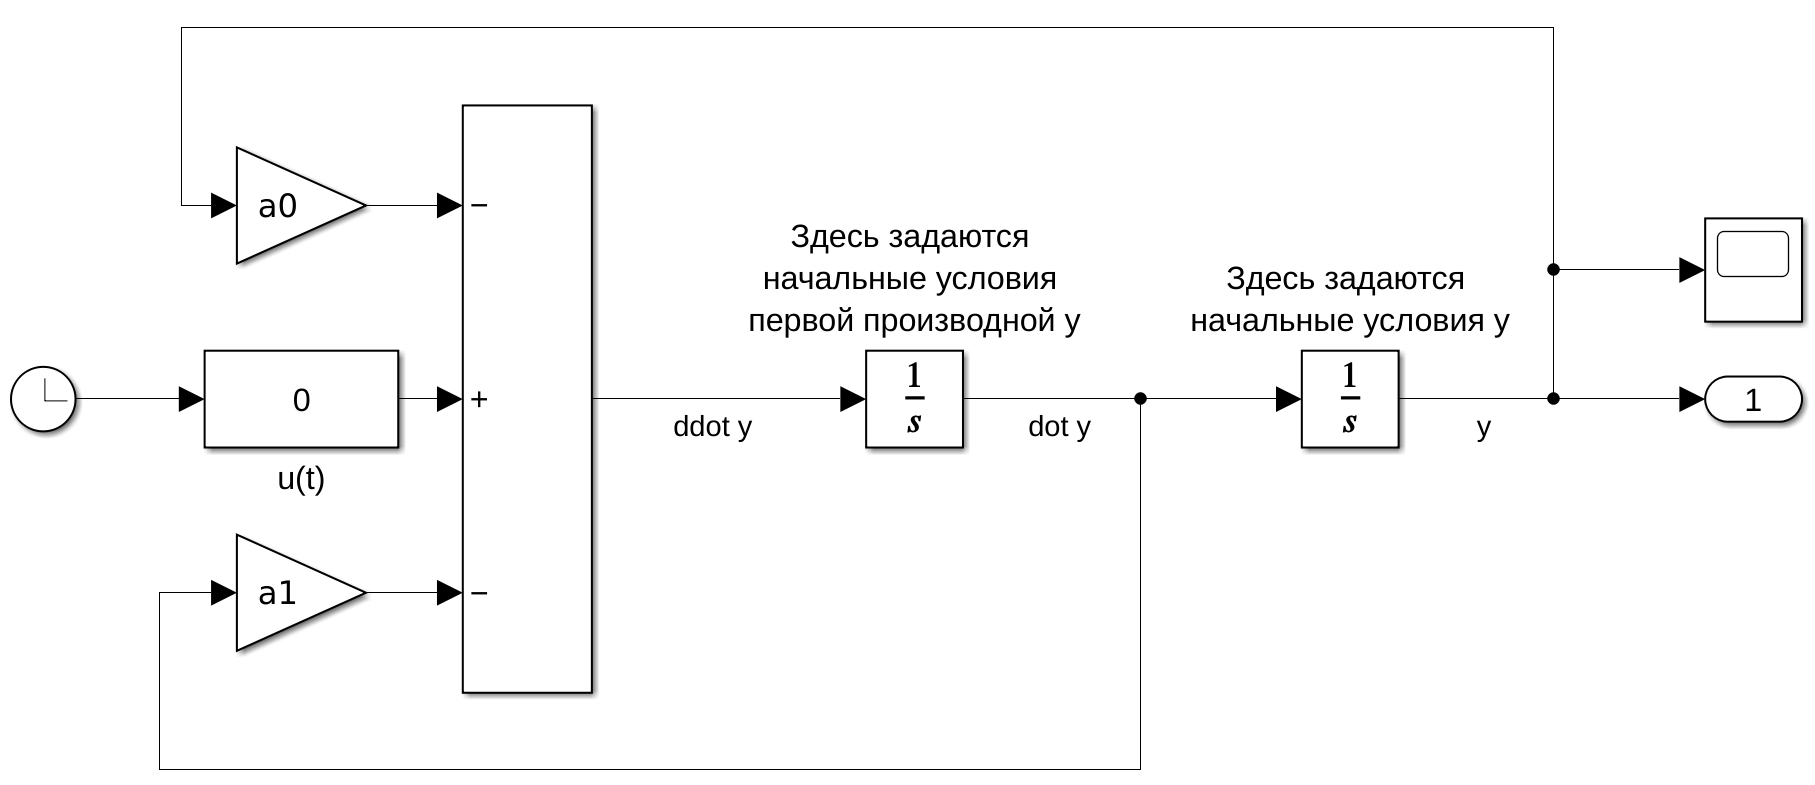
\includegraphics[width=1\textwidth]{figs/task_1_slx.png}
    \caption{Структурная схема диффириального уравнения задания 1.}
    \label{fig:task_1_slx}
\end{figure}
    
\begin{figure}
    \centering
    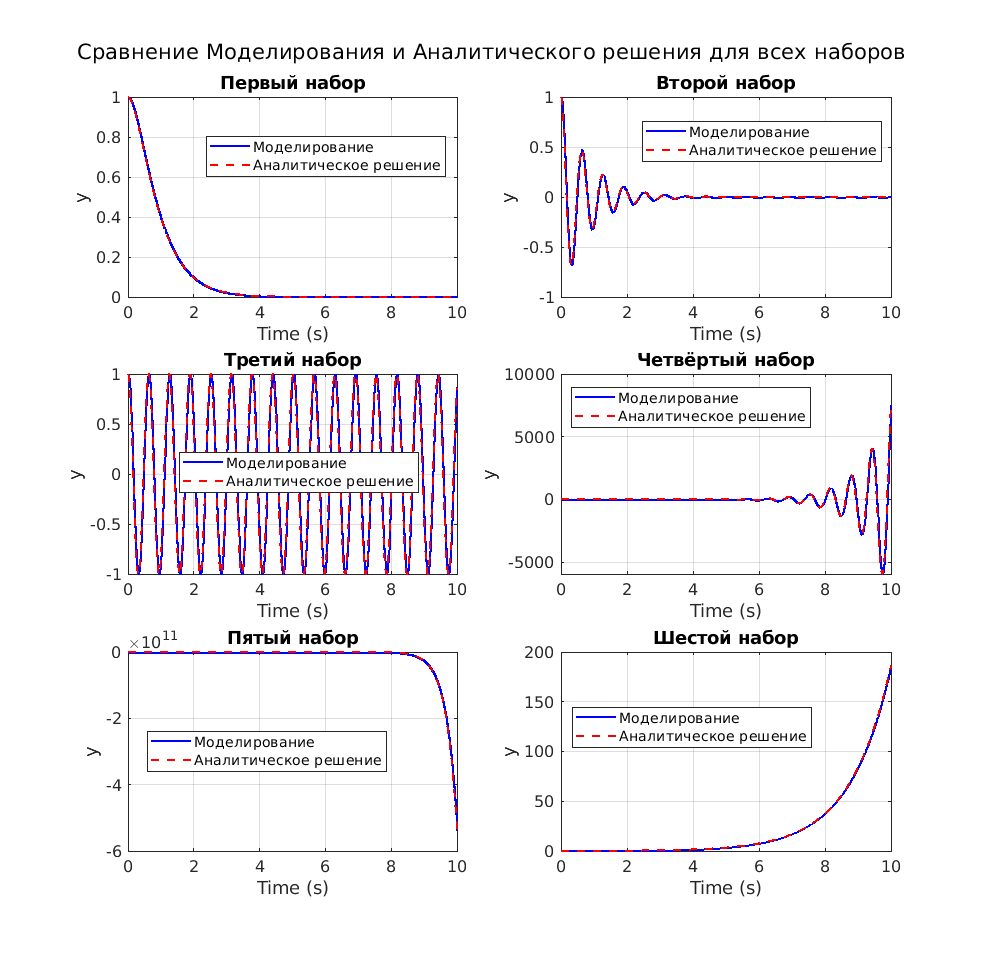
\includegraphics[width=1\textwidth]{figs/task_1_out.png}
    \caption{Графики свободного движения задания 1.}
    \label{fig:task_1_out}
\end{figure}
    